\subsection{Revolving Binary Systems}

Revolving binary systems are a very high energy systems which are formed when two massive objects orbit around their common centre of mass called barycenter. Average total mass of such systems are usually greater than 30 solar masses. And average loss of energy per second by such systems will be every huge which will be converted to gravitational waves. Such systems create gravitational waves by a mechanism called `Inspiral' \cite{van_der_Sluys_2008}. There are four phases in this mechanism. \\

\textbf{Interlocking phase} :- This the longest phase where the bodies come closer and get interlocked by their gravity and start to revolve each other around the barycentre. \\

\textbf{Spiral phase} :- Here the objects start getting close as they revolve. Due to the decrease in the distance between them the orbital energy is decreased and this energy is radiated as gravitational wave. But as they come closer and closer, they loose more and more energy, thus the intensity of gravitational wave increases.\\

\textbf{Merger phase} :- During this phase, the bodies collide by producing immense gravitational waves and merge \cite{article}. \\

\textbf{Ring-down phase} :- Finally, the merged bodies become stable and the gravitational wave intensity decreases exponentially and they stop producing gravitational waves. \\

Revolving binary systems produce compact binary inspiral gravitational waves. This is because the intensity of gravitational waves increases slowly during interlocking phase, and exponentially during the spiral phase, then it reaches a peak in merger phase, and finally it decreases rapidly to zero during ring-down phase. The detectors are capable of recording the signal only for a small range of frequency, So in this wave form, the frequency comes to the detecting range and rapidly goes out of range. Thus the signal strength suddenly increases and stops.

\begin{figure}[h]
    \centering
    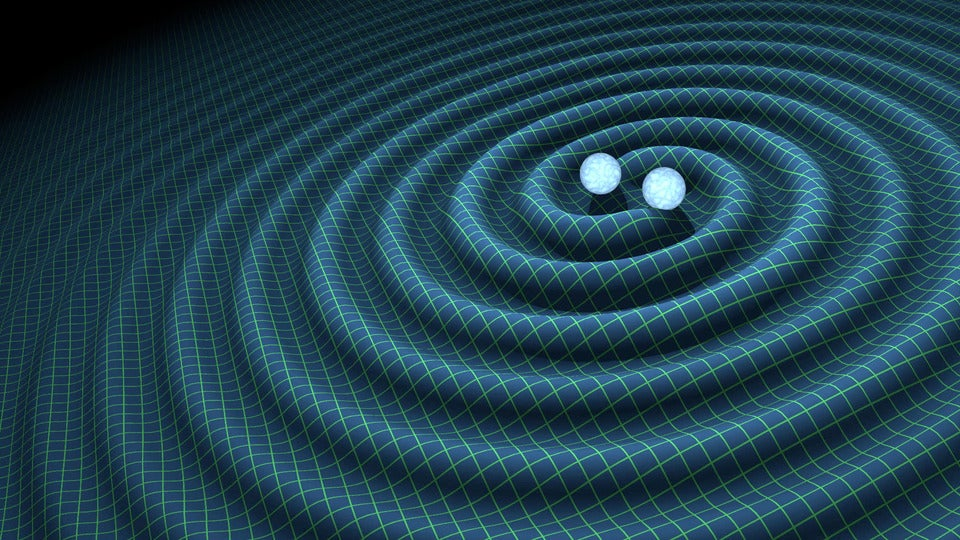
\includegraphics[scale=0.45]{images.tex/binaries.jpeg}
    \caption{Two massive bodies in inspiral mechanism creating gravitational waves \\
    \textbf{Source :-} https://www.scientificamerican.com/article/gravitational-waves-discovered-from-colliding-black-holes1/}
\end{figure}

\pagebreak

\subsubsection{Binary Black Holes (BBH)}

Black holes are massive objects that can warp space-time extensively. If two black holes get closer and start the inspiral mechanism ,they create ripples in space-time and radiate gravitational waves. Such gravitational waves were the first ones to be detected by LIGO in 2015, September 14th. It was estimated that the collision occurred 1.3 billion years ago, thus the merger occurred 1.3 billion light-years away. This merger was named as `\textbf{GW150914}' meaning Gravitational Wave on 15/09/14. This signal lasted for about half a second.

\subsubsection{Binary Neutron Stars (BNS)}

Neutron stars are dense stars formed by the remnants when a massive star explodes as Supernova. So when two neutron stars merge through inspiral mechanism, they can radiate gravitational waves. First BNS merger was detected on 17th August 2017 and this was named as `\textbf{GW170817}', where the merger was analyzed both by Electromagnetic waves (Gamma ray) and gravitational waves. The signal lasted for comparatively longer duration for about 100 seconds, thus the mass was estimated to be lesser than black holes and was recognised as neutron star merge.



\begin{figure}[h]
    \centering
    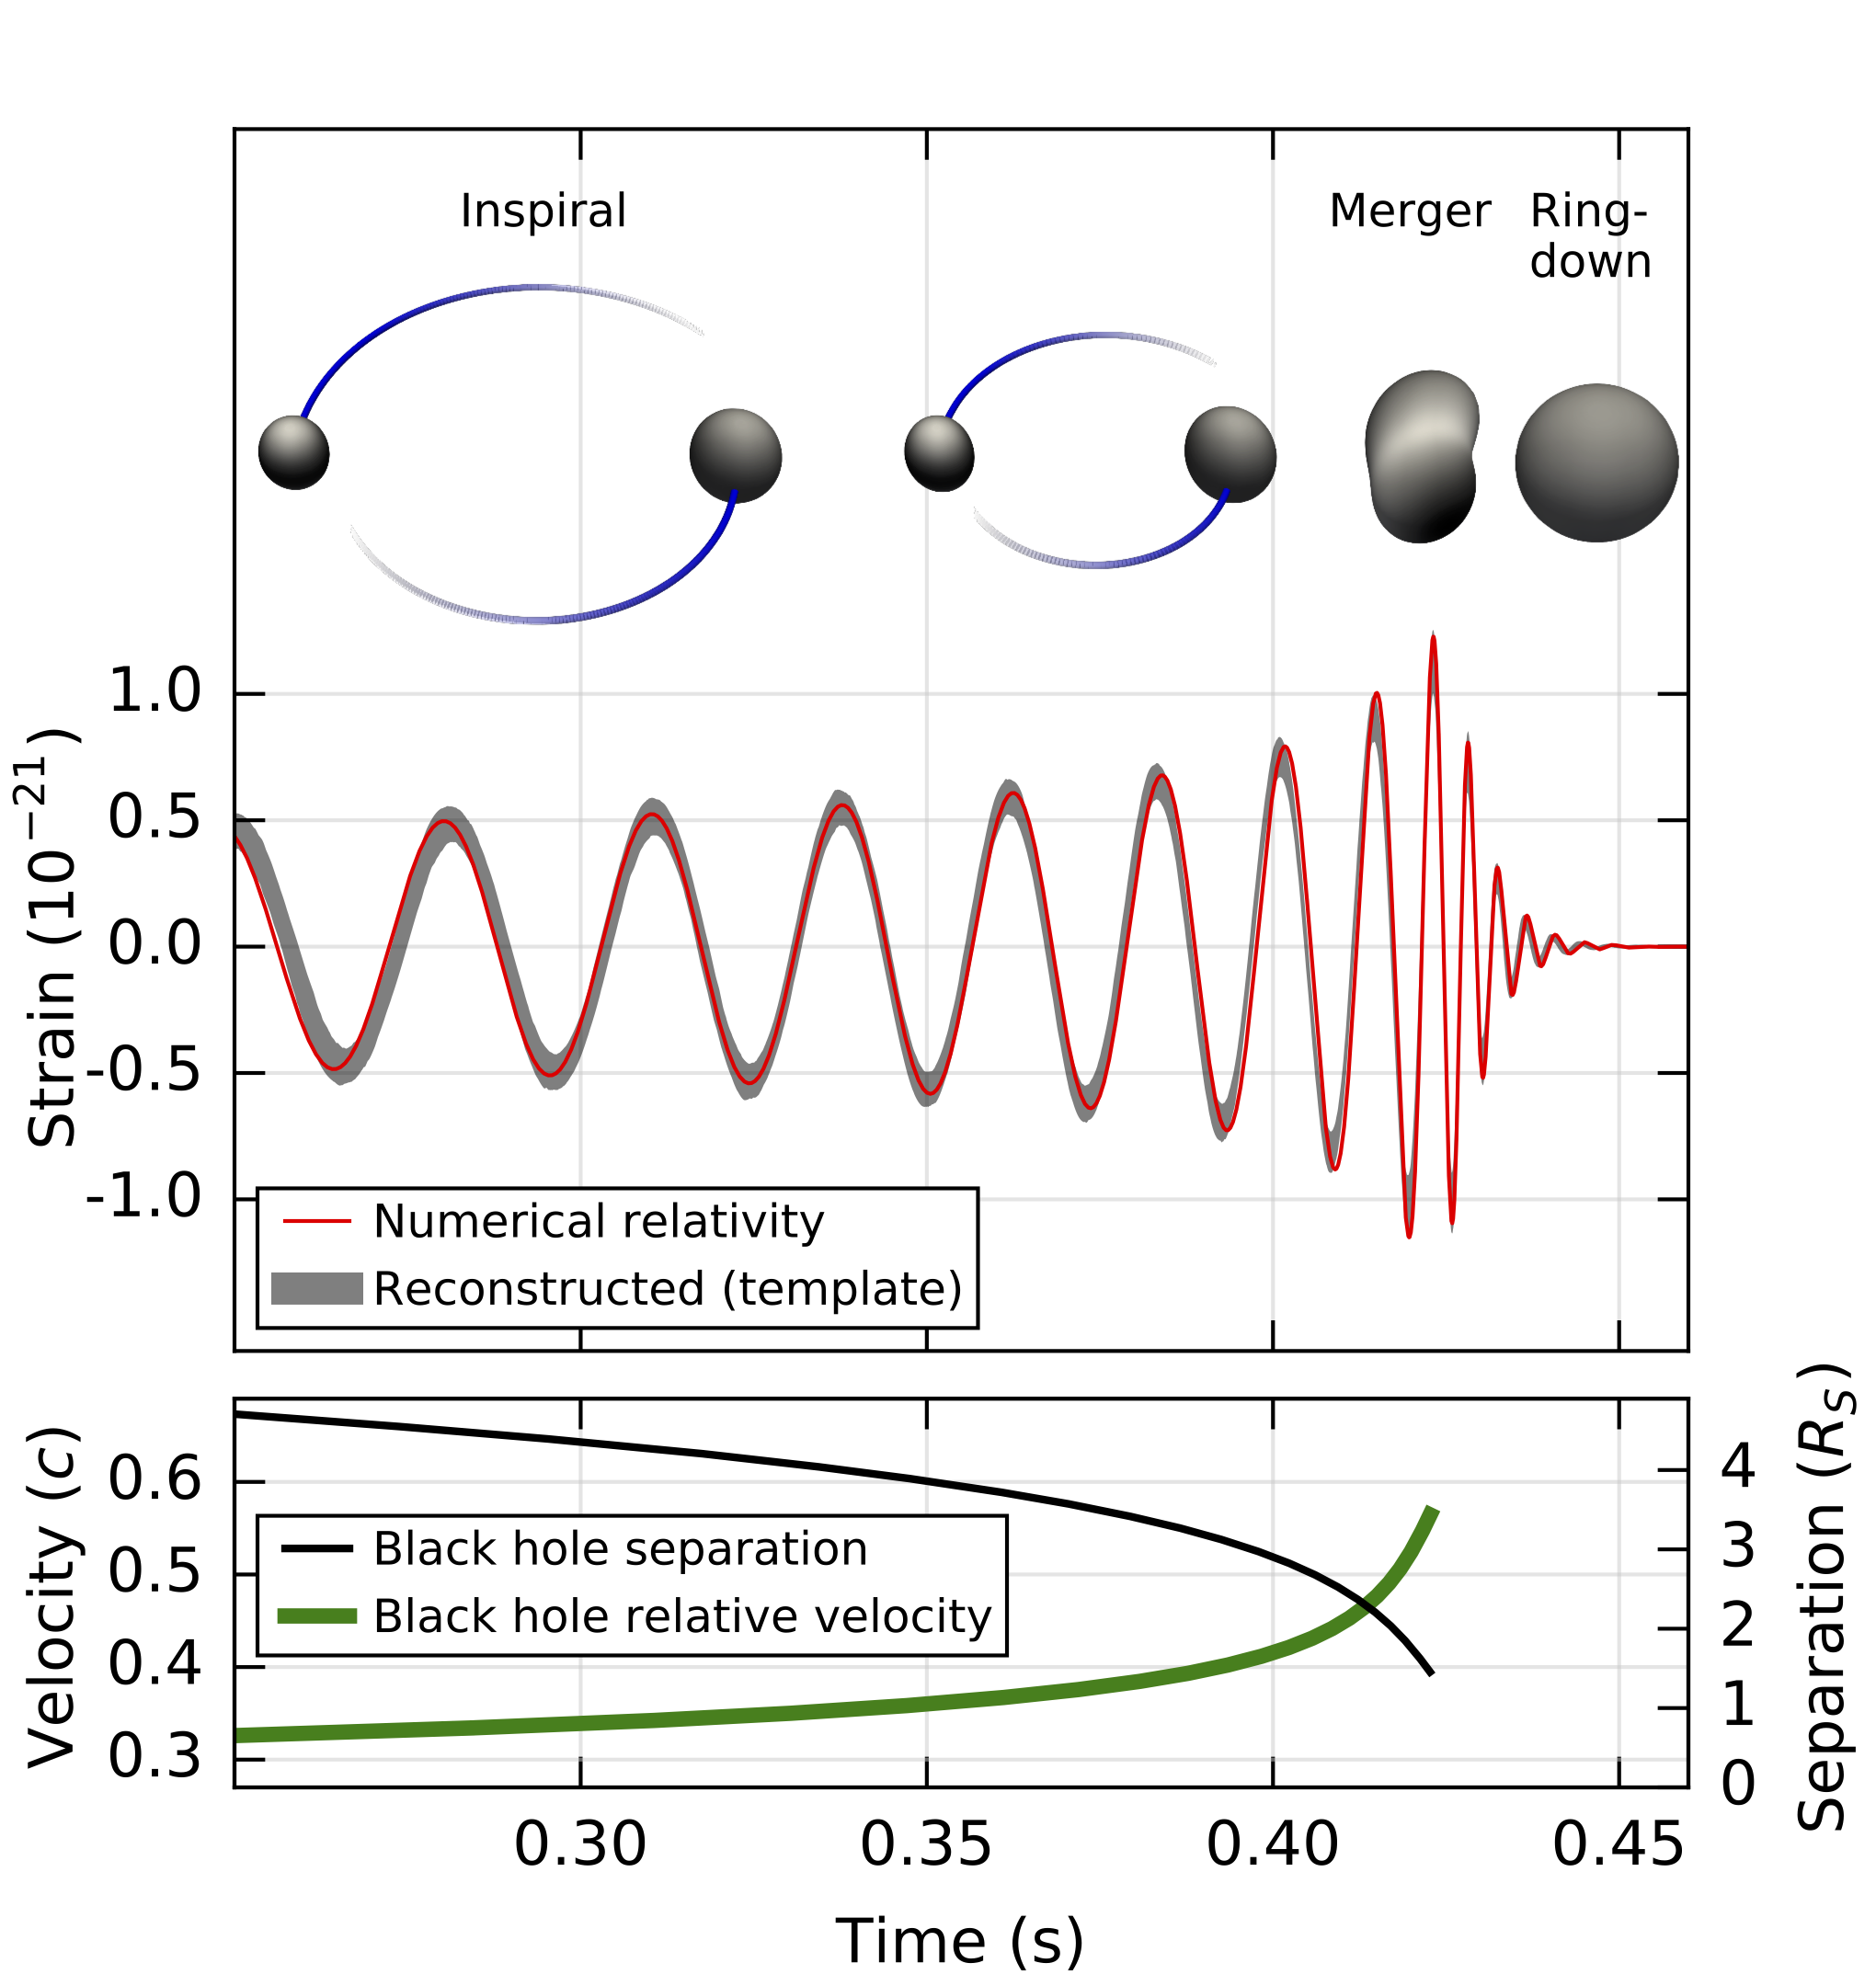
\includegraphics[height = 7cm, width = 8.2 cm]{images.tex/GW150914.png}
    \caption{Characteristics of GW150914   Source:-\url{https://www.ligo.org/science/}}
\end{figure}

\begin{figure}[h]
     \centering
     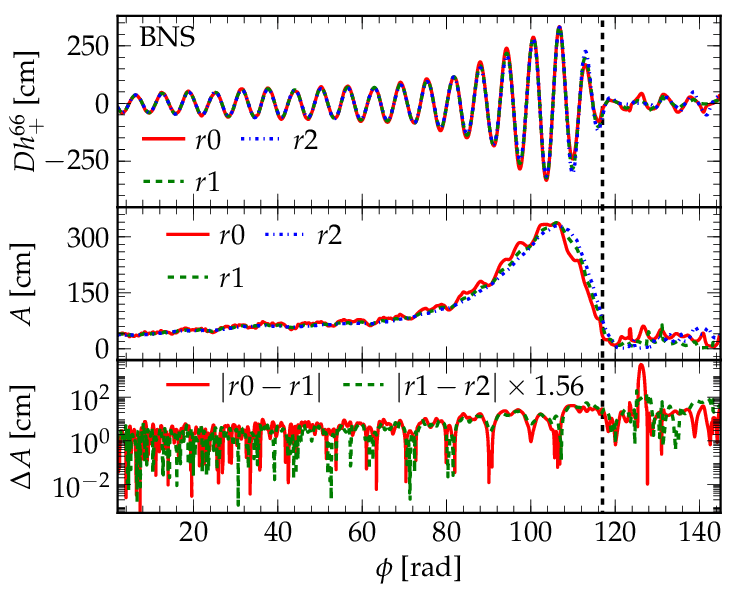
\includegraphics[scale = 0.31]{images.tex/GW170817.png}
     \caption{Characteristics of GW170817\\ Source:- \url{https://www.researchgate.net/publication/233846764}}
\end{figure}

\pagebreak
